
\documentclass[a4paper,UKenglish,cleveref, autoref]{lipics-v2019}
\usepackage{hyperref}
\usepackage{minted} % pip3 install pygments, pdflatex -shell-escape hb
\newminted[elpicode]{elpi.py:ElpiLexer -x}{linenos=true,fontsize=\footnotesize,escapeinside=\%\%}
\newmintinline[elpi]{elpi.py:ElpiLexer -x}{fontsize=\small}
\newminted[coqcode]{elpi.py:CoqElpiLexer -x}{linenos=true,fontsize=\footnotesize,mathescape,escapeinside=\#\#}
\newmintinline[coq]{elpi.py:CoqElpiLexer -x}{fontsize=\small}
\usepackage{xcolor}
\usepackage{wrapfig}

\definecolor{dkgreen}{rgb}{0, 0.502, 0}

\newcommand{\coqelpi}{Coq-Elpi}
\newcommand{\HB}{\ensuremath{\mathcal{HB}}}
\newcommand{\hb}{\coq{hierarchy-builder}}

%This is a template for producing LIPIcs articles.
%See lipics-manual.pdf for further information.
%for A4 paper format use option "a4paper", for US-letter use option "letterpaper"
%for british hyphenation rules use option "UKenglish", for american hyphenation rules use option "USenglish"
%for section-numbered lemmas etc., use "numberwithinsect"
%for enabling cleveref support, use "cleveref"
%for enabling cleveref support, use "autoref"


%\graphicspath{{./graphics/}}%helpful if your graphic files are in another directory

\bibliographystyle{plainurl}% the mandatory bibstyle

\title{Hierarchy Builder: algebraic~hierarchies made easy in Coq with Elpi} %TODO Please add

\titlerunning{Hierarchy Builder}%optional, please use if title is longer than one line

\author{Cyril Cohen}{Inria, France}{Cyril.Cohen@inria.fr}{}{}
\author{Kazuhiko Sakaguchi}{University of Tsukuba, Japan}{sakaguchi@logic.cs.tsukuba.ac.jp}{}{}
\author{Enrico Tassi}{Inria, France}{Enrico.Tassi@inria.fr}{}{}
\authorrunning{C.\,Cohen and K.\,Sakaguchi and E.\,Tassi}
% \author{John Q. Public}{Dummy University Computing Laboratory, [optional: Address], Country \and My second affiliation, Country \and \url{http://www.myhomepage.edu} }{johnqpublic@dummyuni.org}{https://orcid.org/0000-0002-1825-0097}{(Optional) author-specific funding acknowledgements}%TODO mandatory, please use full name; only 1 author per \author macro; first two parameters are mandatory, other parameters can be empty. Please provide at least the name of the affiliation and the country. The full address is optional
% \author{Joan R. Public\footnote{Optional footnote, e.g. to mark corresponding author}}{Department of Informatics, Dummy College, [optional: Address], Country}{joanrpublic@dummycollege.org}{[orcid]}{[funding]}
% \authorrunning{J.\,Q. Public and J.\,R. Public}%TODO mandatory. First: Use abbreviated first/middle names. Second (only in severe cases): Use first author plus 'et al.'

\Copyright{Cyril Cohen and Kazuhiko Sakaguchi and Enrico Tassi}%TODO mandatory, please use full first names. LIPIcs license is "CC-BY";  http://creativecommons.org/licenses/by/3.0/

\ccsdesc[100]{General and reference~General literature}
\ccsdesc[100]{General and reference}%TODO mandatory: Please choose ACM 2012 classifications from https://dl.acm.org/ccs/ccs_flat.cfm
\supplement{Source code of the Coq package: \url{https://github.com/math-comp/hierarchy-builder}}
\keywords{Algebraic Hierarchy, Packed Classes, Coq, Elpi, Metaprogramming, $\lambda$Prolog}%TODO mandatory; please add comma-separated list of keywords

\category{}%optional, e.g. invited paper

\relatedversion{}%optional, e.g. full version hosted on arXiv, HAL, or other respository/website
%\relatedversion{A full version of the paper is available at \url{...}.}

\supplement{}%optional, e.g. related research data, source code, ... hosted on a repository like zenodo, figshare, GitHub, ...

%\funding{(Optional) general funding statement \dots}%optional, to capture a funding statement, which applies to all authors. Please enter author specific funding statements as fifth argument of the \author macro.

%\acknowledgements{I want to thank \dots}%optional

%\nolinenumbers %uncomment to disable line numbering

%\hideLIPIcs  %uncomment to remove references to LIPIcs series (logo, DOI, ...), e.g. when preparing a pre-final version to be uploaded to arXiv or another public repository

%Editor-only macros:: begin (do not touch as author)%%%%%%%%%%%%%%%%%%%%%%%%%%%%%%%%%%
\EventEditors{John Q. Open and Joan R. Access}
\EventNoEds{2}
\EventLongTitle{42nd Conference on Very Important Topics (CVIT 2016)}
\EventShortTitle{CVIT 2016}
\EventAcronym{CVIT}
\EventYear{2016}
\EventDate{December 24--27, 2016}
\EventLocation{Little Whinging, United Kingdom}
\EventLogo{}
\SeriesVolume{42}
\ArticleNo{23}
%%%%%%%%%%%%%%%%%%%%%%%%%%%%%%%%%%%%%%%%%%%%%%%%%%%%%%

% TODO: Write glossary
% remove distinction
% TODO: Structure -> Class
% TODO: packager -> ClassBuilder
% TODO: Builder -> Builder
% Factories ( primitive / general ) ; kill mixin

\newcommand{\Lang}{\ensuremath{\Lambda}}
\newcommand{\term}{term}
\newcommand{\mixin}{mixin}
\newcommand{\mixins}{mixins}
\newcommand{\Mixins}{Mixins}
\newcommand{\M}{\ensuremath{\mathcal{M}}}
\newcommand{\factory}{factory}
\newcommand{\factories}{factories}
\newcommand{\Factories}{Factories}
% \newcommand{\packager}{packager}
% \newcommand{\packagers}{packagers}
% \newcommand{\Packager}{Packager}
\newcommand{\phantterm}{abbreviation}
\newcommand{\phantterms}{abbreviations}
\newcommand{\Phantterms}{abbreviations}
\newcommand{\builder}{builder}
\newcommand{\mixinbuilder}{builder}
\newcommand{\mixinbuilders}{builders}
\newcommand{\factoryinstance}{factory instance}
\newcommand{\factoryinstances}{factory instances}
\newcommand{\F}{\ensuremath{\mathcal{F}}}
\newcommand{\dep}{\ensuremath{\mathit{dep}}}
\newcommand{\powerset}[1]{\raisebox{.15\baselineskip}{\Large\ensuremath{\wp}}(#1)}
\newcommand{\C}{\ensuremath{\mathcal{C}}}
\newcommand{\B}{\ensuremath{\mathcal{B}}}
\newcommand{\class}{class}
\newcommand{\classes}{classes}
\newcommand{\cdef}{\ensuremath{\mathit{def}}}
\newcommand{\Str}{\ensuremath{\mathcal{S}}}
\newcommand{\structure}{structure}
\newcommand{\structures}{structures}
\newcommand{\issubclass}{\ensuremath{\leq}}
\newcommand{\subclass}{subclass}
\newcommand{\join}{\ensuremath{\mathit{join}}}
\newcommand{\requires}{\ensuremath{\mathit{requires}}}
\newcommand{\target}{\ensuremath{\mathit{target}}}
\newcommand{\provides}{\ensuremath{\mathit{provides}}}
\newcommand{\from}{\ensuremath{\mathsf{from}}}
\newcommand{\proj}[2]{\ensuremath{#1[#2]}}
\newcommand{\set}[1]{\left\{#1\right\}}
\newcommand{\enum}[2]{\ensuremath{\set{#1,\ldots,#2}}}
\newcommand{\vect}[1]{\overrightarrow{#1}}
\newcommand{\pmp}[1]{\ensuremath{\vect{\left(p : m\ T\ p_\sigma\right)}^{#1}}}
\newcommand{\hbmixin}{{\tt\color{dkgreen}Elpi hb.mixin}}
\newcommand{\hbfactory}{{\tt\color{dkgreen}Elpi hb.factory}}
\newcommand{\hbinstance}{{\tt\color{dkgreen}Elpi hb.instance}}
\newcommand{\hbstructure}{{\tt\color{dkgreen}Elpi hb.structure}}
\newcommand{\hbend}{{\tt\color{dkgreen}Elpi hb.end}}

\newtheoremstyle{implem}{\topsep}{\topsep}{}{0pt}{\sffamily\bfseries}{ }{5pt plus 1pt minus 1pt}%
{$\blacktriangleright$ \thmname{#1}\thmnumber{ #2}\thmnote{ #3}}

\theoremstyle{implem}
\newtheorem*{implementation}{Implementation of}

\theoremstyle{implem}
\newtheorem*{invariant}{Programming invariant for}

\newtheoremstyle{command}{\topsep}{\topsep}{}{0pt}{\sffamily\bfseries}{ }{5pt plus 1pt minus 1pt}%
{$\blacktriangleright$ \thmname{#1} {\coq{#3}}}
\theoremstyle{command}
\newtheorem*{command}{Coq command}

\begin{document}

\maketitle

%TODO mandatory: add short abstract of the document
\begin{abstract}
It is nowadays customary to organize libraries of machine checked
proofs around hierarchies of algebraic
structures~\cite{DBLP:conf/mpc/AffeldtNS19,DBLP:journals/mics/BoldoLM15,Cohen_phd,Holzl:2013,10.1145/3372885.3373824,Rouhling_phd,mathclasses}.
One influential example is the Mathematical Components library on top
of which the long and intricate proof of the Odd Order
Theorem could be fully formalized~\cite{DBLP:conf/itp/GonthierAABCGRMOBPRSTT13}.

Still, building algebraic hierarchies in a proof assistant such as Coq~\cite{Coq:manual}
requires a lot of manual labor and often a deep expertise in the internals of
the prover~\cite{DBLP:conf/tphol/GarillotGMR09,DBLP:conf/itp/MahboubiT13}.
Moreover, according to our experience~\cite{KSdraft},
making a hierarchy evolve without causing breakage in client code is equally tricky:
even a simple refactoring such as splitting a structure into two simpler ones
is hard to get right.

In this paper we describe \HB{}, a high level language
to \emph{build} hierarchies of algebraic structures and to make these hierarchies
\emph{evolve} without breaking user code. The key concepts are the ones of
\emph{\factory{}}, \emph{\mixinbuilder{}} and \emph{\phantterm{}} that let the hierarchy developer
describe an actual
interface for their library. Behind that interface the developer can provide
appropriate code to ensure retro compatibility.
We implement the \HB{} language in the \hb{} addon for the Coq
system using the Elpi~\cite{DBLP:conf/lpar/DunchevGCT15,CoqElpi}
extension language.
\end{abstract}

%%%%%%%%%%%%%%%%%%%%%%%%%%%%%%%%%%%%%%%%%%%%%%%%%%%%%%%%%%%%%%%%%%%%%%%
\section{Introduction}

Modern libraries of machine checked proofs are organized around
hierarchies of algebraic structures~\cite{DBLP:conf/mpc/AffeldtNS19,DBLP:journals/mics/BoldoLM15,Cohen_phd,Holzl:2013,10.1145/3372885.3373824,Rouhling_phd,mathclasses}.
For example the Mathematical Components library for the Coq system~\cite{Coq:manual}
provides a very rich, ever growing, hierarchy of structures such as
group, ring, module, algebra, field, partial order, order, lattice\ldots
The hierarchy does not only serve the purpose of organizing knowledge, but
also to make it easy to exploit it. Indeed the interactive prover can
take advantage of the structure of the library and the relation between
its concepts to infer part of information usually left implicit
by the user, a capability that turned out to be key to tame
the complexity and size of the formal proof of the Odd Order
Theorem~\cite{DBLP:conf/itp/GonthierAABCGRMOBPRSTT13}.

The hierarchy of the Mathematical Components library
is implemented following the discipline of Packed Classes initially introduced
in \cite{DBLP:conf/tphol/GarillotGMR09} and later also adopted in
\cite{DBLP:conf/mpc/AffeldtNS19} and \cite{DBLP:journals/mics/BoldoLM15}.
We call Packed Classes a discipline, and not a language, because, in spite of
its many virtues, it is unwieldy to use. In particular it leaks to the user
many of the technical details of the Coq system. As a result, one
needs to be a Coq expert in order to build or modify a hierarchy, and even
experts make mistakes as shown in~\cite{KSdraft}.
Another inconvenience of the Packed Classes discipline is that even
simple changes to the hierarchy, such as splitting a structure into
two simpler ones, break user code.

In this paper we describe \HB{}, a high level language
to \emph{build} hierarchies of algebraic structures and to make these hierarchies
\emph{evolve} without breaking user code. The key concepts are the ones of
\emph{\factory{}} and \emph{\phantterm{}} that let the hierarchy developer describe an actual
interface for their library. Behind that interface the developer can provide
appropriate code to ensure retro compatibility.
We implement the \HB{} language by compiling it
to a variant of the Packed Classes discipline, that we call \emph{flat},
in the \hb{} addon for Coq. We write this addon using the
Elpi~\cite{DBLP:conf/lpar/DunchevGCT15,CoqElpi} extension language.\\

\noindent To sum up, the main contributions of the paper are:
\begin{itemize}
\item the design of the \HB{} language,
\item the compilation of \HB{} to the (flat) Packed Classes discipline, and
\item the implementation of \HB{} in the \hb{} addon for Coq.
\end{itemize}
The paper is organized as follows. Via an example we introduce
\HB{} and its key ideas. %We then provide a formal description of \HB{}.
We then describe the discipline
of Packed Classes and we show how \HB{} can be compiled to it.
We then discuss the implementation of the Coq addon via the Elpi extension
language and we position \HB{} in the literature.

%%%%%%%%%%%%%%%%%%%%%%%%%%%%%%%%%%%%%%%%%%%%%%%%%%%%%%%%%%%%%%%%%%%%%%%%5
\section{\HB{} by examples: building and evolving a hierarchy}
\label{sec:example}

The first version of our hierarchy (that we name V1) features only two
structures: \coq{Monoid} and \coq{Ring}.
%\marginpar{remove hb.end for \mixins{}, use next release of coq elpi}
\begin{coqcode}
#\hbmixin{}# Monoid_of_Type A.                       #\label{demo:mixin:mot}#
  Record axioms := {
    zero : A;
    add : A -> A -> A;
    addrA : associative add;             (* `add` is associative.                   *)
    add0r : left_id zero add;            (* `zero` is the left and right neutral    *)
    addr0 : right_id zero add;           (*   element with respect to `add`.        *)
  }.
#\hbend{}#.                                              #\label{demo:mixin:mot:end}#
#\hbstructure{}# Monoid Monoid_of_Type.axioms.        #\label{demo:structure:monoid}#

#\hbmixin{}# Ring_of_Monoid A Monoid.axioms.       #\label{demo:mixin:rom}#
  Record axioms := {
    one : A;
    opp : A -> A;
    mul : A -> A -> A;
    addNr : left_inverse zero opp add;   (* `opp x` is the left and right additive  *)
    addrN : right_inverse zero opp add;  (*   inverse of `x`.                       *)
    mulrA : associative mul;             (* `mul` is associative.                   *)
    mul1r : left_id one mul;             (* `one` is the left and right neutral     *)
    mulr1 : right_id one mul;            (*   element with respect to `mul`.        *)
    mulrDl : left_distributive mul add;  (* `mul` is left and right distributive    *)
    mulrDr : right_distributive mul add; (*   over `add`.                           *)
  }.
#\hbend{}#.
#\hbstructure{}# Ring Monoid.axioms Ring_of_Monoid.axioms. #\label{demo:structure:ring}#

\end{coqcode}

In order to build a structure we need to declare some \factories{} and
later assemble them. One kind of \factory{} supported by \HB{}, the simplest
one, is called \emph{\mixin{}} and is embodied by a record, by convention named
\coq{axioms}, that gathers operations and properties.

\Mixins{} are declared via the \hbmixin{} command
that takes a module name,
a type variable name and a possibly empty list of \factories{} for that type.
The code between lines~\ref{demo:mixin:mot}
and~\ref{demo:mixin:mot:end} declares a \mixin{} that can turn a naked
type \coq{A} into a monoid, hence we chose the module name to be \coq{Monoid_of_Type}.

The \hbstructure{} command takes in input a name S and a possibly
empty list of \factories{}.
It registers a structure S in the hierarchy placing
any definition specific to that structure inside a Coq module named \coq{S}.
Line~\ref{demo:structure:monoid} hence forges the \coq{Monoid} structure.

Line~\ref{demo:mixin:rom} declares a second \mixin{} collecting the operations
and properties that are needed in order to enrich a monoid to a ring, hence
the name \coq{Ring_of_Monoid}. Indeed this time the type variable \coq{A}
is followed by \coq{Monoid.axioms} that enriches
\coq{A} with the operations and properties of monoids. As a consequence
\coq{add} and \coq{zero} can be used to express the new properties.

The last line declares the \coq{Ring} structure to hold all the axioms declared
so far. We can now inspect the contents of the hierarchy and then
proceed to build a theory about abstract rings,
register examples (instances) of ring structures
and finally use the abstract theory on these examples.

\begin{coqcode}
Print Monoid.type. (* Monoid.type  :=  { sort : Type;  ... }                           *) #\label{demo:theory:print:type}#
Check @add.        (* add          :   forall M : Monoid.type, M -> M -> M             *) #\label{demo:theory:check:add}#
Check @addNr.      (* addNr        :   forall R : Ring.type, left_inverse zero opp add *) #\label{demo:theory:check:addNr}#

Lemma addrC : forall R : Ring.type, commutative (@add R).                       #\label{demo:theory:state:addrC}#
Proof. (* Proof by Hankel 1867, omitted for brevity *) Qed.

Definition Z_Monoid_axioms : Monoid_of_Type.axioms Z :=                         #\label{demo:theory:z:monoid:axioms}#
  Monoid_of_Type.Axioms Z 0 Z.add Z.add_assoc Z.add_0_l Z.add_0_r.

#\hbinstance{}# Z Z_Monoid_axioms.                                            #\label{demo:theory:z:monoid:canonical}#

Definition Z_Ring_axioms : Ring_of_Monoid.axioms Z _ :=                        #\label{demo:theory:z:ring:axioms}#
  Ring_of_Monoid.Axioms Z 1 Z.opp Z.mul
    Z.add_opp_diag_l Z.add_opp_diag_r Z.mul_assoc Z.mul_1_l Z.mul_1_r
    Z.mul_add_distr_r Z.mul_add_distr_l.

#\hbinstance{}# Z Z_Ring_axioms.                                              #\label{demo:theory:z:ring:canonical}#

Lemma exercise (m n : Z) : (n + m) - n * 1 = m.
Proof. by rewrite mulr1 (addrC n) -(addrA m) addrN addr0. Qed.
\end{coqcode}

We can print the type for monoids as forged by \HB{} (line~\ref{demo:theory:print:type}).
It packs a carrier, called \coq{sort}, and the collection of operation and
properties that we omit for brevity.  We can also look at the type of two
constants synthesized by \HB{} out of the hierarchy declaration. Remark that
while the names of the constants come from the names of \mixin{} fields,
their types differ.
In particular they are quantified over a \coq{Monoid.type} or \coq{Ring.type},
and not a simple type \coq{A} as in the \mixins{}. Moreover we evince that
the \coq{sort} projection is declared as an implicit coercion~\cite{Saibi97}
and is automatically inserted in order to make \coq{M -> M -> M} a meaningful
type for binary operations on the carrier of \coq{M}. Last, we see that
properties are quantified on (hence apply to) the structure they belong to but
use, in their statements, operations belonging to simpler structures.
For example \coq{addNr} is a property of a ring but  its statement mentions \coq{add},\
the operation of the underlying monoid.

We then follow the proof of Hankel~\cite{nearrings} to show that
ring axioms imply the commutativity of the underlying monoid
(line~\ref{demo:theory:state:addrC}). This simple example shows we can
populate the theory of abstract rings with new results.

We use the \coq{Monoid_of_Type.Axioms} \emph{\phantterm{}}
(line~\ref{demo:theory:z:monoid:axioms})
in order to build an instance of the \coq{Monoid}
structure for binary integers \coq{Z}.
We then register that monoid instance as the canonical one on \coq{Z}
(line~\ref{demo:theory:z:monoid:canonical}) via the command
\coq{hb.canonical}.
We can similarly declare that \coq{Z} forms a ring by using
the \coq{Ring_of_Monoid.Axioms} \phantterm{}
(lines~\ref{demo:theory:z:ring:axioms} and~\ref{demo:theory:z:ring:canonical}).
Note that the \coq{Ring_of_Monoid.Axioms} \phantterm{} is not
a plain record constructor for \coq{Ring_of_Monoid.axioms}, since that
would require more arguments, namely the monoid ones (see the \coq{_}
at line~\ref{demo:theory:z:ring:axioms}). The
\phantterm{} synthesized by \HB{} infers them automatically
(as in~\cite[Section 7]{DBLP:conf/itp/MahboubiT13}) thanks to the \coq{hb.canonical}
declaration given just above.

From now on the axioms as well as the abstract theory of rings apply to
integers, as shown in lemma \coq{exercise}. The details of the proof
do not matter here, what is worth pointing out is that in a single
statement we mix monoid (e.g. \coq{+}) and ring (e.g. \coq{-}) operations and in the
proof we use monoid axioms (e.g. \coq{addrA}), ring axioms
(e.g. \coq{addrN}) and ring lemmas (e.g. \coq{addrC}), all seamlessly.

\subsection{Evolution of the hierarchy}\label{subsec:evolution}

We proceed by accommodating the intermediate
structure of Abelian groups.

\begin{coqcode}
#\hbmixin{}# Monoid_of_Type A.
  Record axioms := { ... (* unchanged *) ... }.
#\hbend{}#.
#\hbstructure{}# Monoid Monoid_of_Type.axioms.

#\hbmixin{}# AbelianGroup_of_Monoid A Monoid.axioms.
  Record axioms := {
    opp : A -> A;
    addrC : commutative (add : A -> A -> A);
    addNr : left_inverse zero opp add;
  }.
#\hbend{}#.
#\hbstructure{}# AbelianGroup Monoid.axioms AbelianGroup_of_Monoid.axioms.

#\hbmixin{}# Ring_of_AbelianGroup A AbelianGroup.axioms.
  Record axioms := {
    one : A;
    mul : A -> A -> A;
    mulrA : associative mul;
    mul1r : left_id one mul;              mulr1 : right_id one mul;
    mulrDl : left_distributive mul add;   mulrDr : right_distributive mul add;
  }.
#\hbend{}#.
#\hbstructure{}# Ring AbelianGroup.axioms Ring_of_AbelianGroup.axioms.

Lemma addrN {R : AbelianGroup.type} : right_inverse zero opp add.               #\label{demo2:proof:addrN}#
Proof. by move=>x; rewrite addrC addNr. Qed.
\end{coqcode}

Some operations and properties were moved from the old \mixin{} for rings
into a newborn \mixin{} \coq{AbelianGroup_of_Monoid} that gathers the
axioms needed to turn a monoid into an Abelian group. Consequently the \mixin{}
for rings is now called \coq{Ring_of_AbelianGroup} (instead of \coq{Ring_of_Monoid})
since it expects the type \coq{A} to be already an Abelian group and hence
gathers fewer axioms. \\
While operations moved from one structure to another, some properties
undergo a deep change in their status.
The lemma \coq{addrC} part of the abstract theory of
rings is now an axiom of Abelian groups, while \coq{addrN} is no more
an axiom of rings, but rather a theorem of the abstract theory of Abelian
groups.

With this new version of the hierarchy, that we name V2, code written
for version V1 breaks. For example the declaration of the canonical ring over
the integers fails, if only
because we do not have a \coq{Ring_of_Monoid.Axioms} \phantterm{} anymore.

Our objective is to obtain a version of the hierarchy, that we name V3, that does
not only feature Abelian groups but that is also backward compatible
with V1.

\subsection{The missing puzzle piece}\label{subsec:v3}

\begin{figure}[!h]
  \begin{center}
    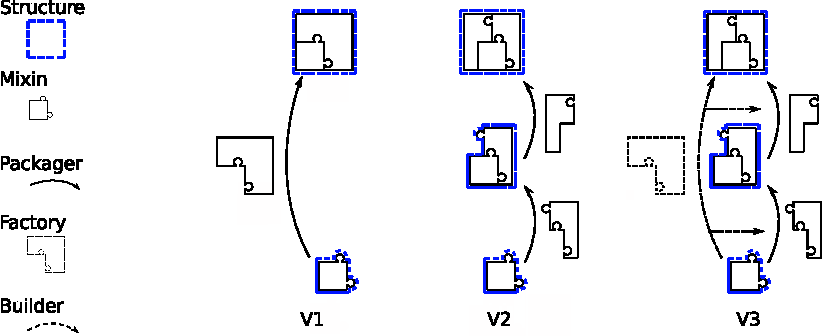
\includegraphics[width=0.8\textwidth]{puzzle.pdf}
  \end{center}
  \caption{\label{fig:puzzle}The evolution of the hierarchy. V3 is backward compatible with V1, while V2 is not.}
\end{figure}

The key to make a hierarchy evolve without breaking user code is the full
fledged notion of \emph{\factory{}} (the \mixins{} seen so far are degenerate,
trivial, \factories{}).
\Factories{}, like \mixins{}, are packages for operations and properties but are
not directly used in the definition of structures. Instead a \factory{} is
equipped with \emph{\builder{}s}: user provided pieces of code that extract
from the \factory{} the contents of \mixins{}, so that existing
\phantterm{}s can be used.

As depicted in figure~\ref{fig:puzzle} we change again the hierarchy
by declaring a \coq{Ring_of_Monoid} \factory{}, that, from the user point of view,
will look indistinguishable from the old \coq{Ring_of_Monoid} \mixin{}
and hence grant backward compatibility between version V3 and version V1.

\begin{coqcode}
#\hbfactory{}# Ring_of_Monoid A Monoid.axioms.
  Record axioms := { ... (* unchanged, see page 2 line 13 *) ... }.

  Variable f : axioms.                                                          #\label{demo3:variable:f}#

  Lemma addrC : commutative add. Proof. (* The same proof as before *) Qed.

  Definition to_AbelianGroup_of_Monoid :=
    AbelianGroup_of_Monoid.Axioms A (opp f) addrC (addNr f). (* addrN unused *)
  #\hbinstance{}# A to_AbelianGroup_of_Monoid.

  Definition to_Ring_of_AbelianGroup :=
    Ring_of_AbelianGroup.Axioms A (one f) (mul f)
      (mulrA f) (mul1r f) (mulr1 f) (mulrDl f) (mulrDr f).
  #\hbinstance{}# A to_Ring_of_AbelianGroup.

#\hbend{}#.
\end{coqcode}

The record \coq{Ring_of_Monoid.axioms} is the same we declared as a \mixin{}
in version V1. In order to make a \factory{} out of it we equip it with
two definitions that embody the \emph{\builder{}s}.
The first is \coq{to_AbelianGroup_of_Monoid} and
explains how to build an \coq{AbelianGroup} structure out of the \factory{}
axioms (named \coq{f}, line~\ref{demo3:variable:f}).
This construction is also registered as canonical for \coq{A},
so that the next construction \coq{to_Ring_of_AbelianGroup} can call
the \coq{Ring_of_AbelianGroup.Axioms} \phantterm{} that requires \coq{A} to be
an \coq{AbelianGroup}.
It is worth pointing out that the proof of \coq{addrC} we had in V1 is now
required in order to write the \builder{} for Abelian groups, while
the \coq{addrN} field is not used (the same statement is already part of
the theory of Abelian groups, see line~\ref{demo2:proof:addrN} of the previous
code snippet).

Thanks to this \factory{} we can now declare \coq{Z} to be an instance
of a ring using the \coq{Ring_of_Monoid.Axioms} \phantterm{}.
The associated \builder{}s generate, behind the scenes, instances of the
\coq{Ring_of_AbelianGroup.axioms} and \coq{AbelianGroup_of_Monoid.axioms} \mixins{}
that in turn are used to build instances of the \coq{AbelianGroup} and \coq{Ring}
structures. Indeed, when used in the context of the hierarchy version V3,
the command \hbinstance{} \coq{Z Z_Ring_axioms}
makes \coq{Z} an instance of \emph{both} structures, and not just the \coq{Ring}
one as in version V1.
Thanks to that the proof of \coq{example} can use the theory of
both structures, for example \coq{addrC} holds on Abelian groups,
\coq{addrA} holds on monoids, while \coq{addr1} holds on rings.
As a result the very same proof works on both
version V1 and V3.

Last, it is worth pointing out that the new \factory{} makes the following
two lines equivalent (the former declares
rings in V1) since they both describe the same set of \mixins{}.

\begin{coqcode}
#\hbstructure{}# Ring Monoid.axioms Ring_of_Monoid.axioms.
#\hbstructure{}# Ring AbelianGroup.axioms Ring_of_AbelianGroup.axioms.
\end{coqcode}

This is another example of client code that would not break: the client of the hierarchy is allowed to declare new
structures on top of existing ones.

\subsection{\HB{} in a nutshell}

By using \HB{} the hierarchy designer has the following freedoms and advantages.

\begin{itemize}
\item Operations and properties (axioms) are made available to the user
      as soon as they are used in a structure. The hierarchy designer
      is free to move them from one to another and replace an axiom
      by a lemma and vice versa.
\item Structures cannot disappear but the way they are built may change.
      The hierarchy designer is free to split structures into smaller
      ones in order to better factor and reuse parts of the hierarchy
      and the library that follows it.
\item \Mixins{} cannot disappear but can change considerably
      in their implementation. A \mixin{} can become a full fledged
      \factory{} equipped with \builder{}s to ensure retro compatibility.
\item \HB{} high level commands compile to
      the discipline of Packed Classes (Coq modules, records, coercions,
      implicit arguments, canonical structure instances, notations,
      \phantterms{}).
      This process lifts a considerable
      burden from the shoulders of the hierarchy designer and the final user
      who are no longer required to master the details of Packed Classes.
\end{itemize}

%%%%%%%%%%%%%%%%%%%%%%%%%%%%%%%%%%%%%%%%%%%%%%%%%%%%%%%%%%%%%%%%%%%%%%%%%%%
\section{\HB{} language}\label{sec:language}

The Coq terms handled by \HB{} are subdivided in five categories, the
\mixins{} \(\M{}\), the \factories{}~\(\F{}\), \mixinbuilders{}
\(\B{}\), the \classes{} \(\C{}\) and the \structures{}
\(\Str{}\). \Mixins{}, \factories{} and instances are tagged by the
user, through the commands \hbmixin{}, \hbfactory{} and \hbinstance{},
and the user may rely on their implementation. However structures and
classes are generated with the command \hbstructure{} and builders are
generated when using \hbinstance{} while declaring a \factory{}, and
the user may only refer to structure types, but should never rely on
their implementation, neither should they rely on explicit builders.

\subsection{\HB{} \mixins{}, \factories{} and instances}
\label{sec:hb-mixins-factories}

\begin{definition}[\M{}, \mixins{}]
A \emph{\mixin{}} \(m \in \M{}\) is a Coq record with one or more parameters.
The first parameter must be a \coq{(T : Type)}, while the other parameters
are \mixins{} applied to \coq{T} and possibly $n$ other distinct \mixins{}. I.e.
\begin{coqcode}
Record #$m$# (T : Type) #\(\pmp{n}\)# : Type := { .. }.
\end{coqcode}
where \(\pmp{n} = \vect{\left(p_i : m_i\ T\ p_{\sigma(i,1)}\ \ldots\ p_{\sigma(i,n_i)}\right)}_{i \in \enum1n}\).
For all \(i \in \enum1n\) we have \(m_i \in \M{}\) and its
arguments consist in $n_i$ of the previously quantified
mixin parameters $p_k$, i.e. for all \(k \in \enum1{n_i}\), we
have \(\sigma(i,k) \in \enum1{i-1}\).
\end{definition}

\begin{definition}[\dep{}, \mixin{} dependencies]
  Given \(m \in \M{}\), we define \(\dep{}(m) \in \powerset\M{}\)
  as the set of all \mixins{} that occur as parameters of \(m\), i.e.
  \(\dep{}(m) = \enum{m_1}{m_n}\).
\end{definition}

\begin{remark}For all \(i \in \enum1n\), we have
\(\dep{}(m_i) = \enum{m_{\sigma(i,1)}}{m_{\sigma(i,m_i)}}\).
\end{remark}

\begin{definition}If \(f : \mathcal{X} \to \powerset{\mathcal{Y}}\), then
\(f^\star : \powerset{\mathcal{X}} \to \powerset{\mathcal{Y}}\) is defined as
\(f^\star(X) = \bigcup_{x \in X} f(x).\)
\end{definition}

\begin{proposition}
\dep{} is transitively closed since records are well typed in the
empty context and describes a DAG since Coq does not admit circular
definitions: \(\dep{}^\star(\dep{}^\star(M)) \subseteq \dep{}^\star(M)\)
\end{proposition}

\begin{definition}[\factories{} \F{}, \mixinbuilders{} \B{} and \from{}]
  A \emph{\mixinbuilder{}} \(\mu \in \B{}\) is any function which parameters are the carrier
  type \coq{(T: Type)}, an arbitrary number of distinct \mixins{}
  \(\enum{m_1}{m_n}\) and an additional argument \(f\), which we call
  a \emph{\factory{}}, and which depends on the \mixins{}. Its return type is
  a \mixin{} \(m_{n+1} \in \M{}\) i.e.
\begin{coqcode}
Definition f (T : Type) #$\pmp{n}$# : Type := ...
Definition #$\mu$# (T : Type) #$\pmp{n}$#: #\(f\ T\ p_1 \ldots p_n\)# -> #\(m_{n+1}\ T\ p_{\sigma(n+1,1)}\ \ldots\ p_{\sigma(n+1,n_i)}\)# := ...
\end{coqcode}

  We define \(\from{} (f, m_{n+1}) = \mu\) to be the (unique) \mixinbuilder{}
  for \(m_{n+1}\) from the \factory{} \(f\).
\end{definition}

\begin{definition}[$\provides{}$, $\requires{}$]
  We define the following functions \begin{itemize}
  \item\( \requires{}(f) = \enum{m_1}{m_n}  \in \powerset\M{}\)
    is the set of mixins a \factory{} \(f \in \F{}\) depends on.
    As a consequence all the
    \mixinbuilders{} of a given \factory{} have the same set of
    dependencies.
  \item\( \provides{}(f) = \{m | \from{}(f,m) \textrm{ is defined}\}
    \in \powerset\M{}\) the set of mixins that a factory
    \(f \in \F{}\) provides, through its \mixinbuilders{}.
  \end{itemize}
Moreover the following properties hold for all \(f \in \F{}\):
  %\begin{proposition}
  %  They validate the following properties for all \(f \in \F{}\):
    \begin{enumerate}
      \item\( \dep{}^\star(\requires{}(f)) \subseteq \requires{}(f)\)
      \item\( \requires{}(f) \cap \provides{}(f) = \emptyset \)
      \item\( \forall m \in \provides{}(f),~ \from{}(f,m) \) is defined
    \end{enumerate}
  %\end{proposition}
\end{definition}

\Mixins{} are declared by the user as the fundamental building blocks of
a hierarchy. As the next proposition shows they shall not be distinguished
from regular \factories{}, since they are a special cases.

\begin{proposition}[\( \M{} \subseteq \F{} \)] For all \(m \in \M{}\)
  we have \(\requires{}(m) = \dep{}(m)\), \(\provides{}(m) = \{m\}\)
  and
  \(\from{}(m,m) = \left(\coq{fun T }\ \pmp{n} \ \coq{(x :}\ m\
  \coq{T }\ p_1\ \ldots p_n\ \coq{) => x}\right) \in \B{}.\)
\end{proposition}


\begin{command} to declare a new mixin:
\begin{coqcode}
#\hbmixin{}# M T #$f_1\ \ldots\ f_n$#. Record axioms := { .. }. #\hbend{}#.
\end{coqcode}
  Creates a module \coq{M} with a record
  \coq{M.axioms}, which depends on the \mixins{}
  \(\requires{}(\coq{M.axioms}) =
  \provides{}^\star\left(\enum{f_1}{f_n}\right)\), and registers this
  new record both as a \mixin{} and a \factory{}. It also creates a
  \phantterm{} \coq{M.Axioms.}
\end{command}

\begin{command} to declare an instance: \hbinstance{}
  \(X\ b_1 \ldots b_k\), synthesizes terms corresponding to all the
  \mixins{} that can be built from the $b_i$. Indeed if
  \(b_i : f_i\ T\ \ldots\), then this command creates elements of type
  \(\provides{}^\star\left(\enum{f_1}{f_k}\right).\) This command also
  generates unification hints as described in
  Section~\ref{sec:target-lang}.
\end{command}

\begin{command} to declare a new \factory{} and generate new \mixinbuilders:
\begin{coqcode}
#\hbfactory{}# M T #$f_1\ \ldots\ f_n$#.
  Record axioms := { .. }.
  Variable (a : axioms _).

  Definition #$b_{n+1}$# : #$f_{n+1}$# T .. := ...
  #\hbinstance{}# T #$b_{n+1}$#.
  ..
  Definition #$b_{n+k}$# : #$f_{n+k}$# T .. := ...
  #\hbinstance{}# T #$b_{n+k}$#.
#\hbend{}#.
\end{coqcode}
  Creates a module \coq{M} with a record
  \coq{M.axioms}, which depends on the mixins
  \(\requires{}(\coq{M.axioms}) =
  \provides{}^\star\left(\enum{f_1}{f_n}\right)\) and registers this
  new record as a factory. We then use the \factoryinstances{}
  \(b_{n+1}, \ldots, b_{n+k}\) provided by the user and derive
  \mixinbuilders{} from them, so that
  \(\provides{}(\coq{M.axioms}) = \provides{}^\star\left(\enum{f_{n+1}}{f_{n+k}}\right).\)

  It is thus necessary that
  \(\requires{}^\star\left(\enum{f_{n+1}}{f_{n+k}}\right) \subseteq
  \provides{}^\star\left(\enum{f_1}{f_n}\right).\)
\end{command}

Note that the \(b_i\) are not \mixinbuilders{} since their return types
are not necessarily \mixins{}, but could be a \factory{}. However, since all
\factories{} provide \mixin{} through \mixinbuilders{}, we can
obtain \mixinbuilders{} out of each \(b_i\) by function composition.

\subsection{\HB{} classes and structures}
\label{sec:hb-class-struct}


\begin{definition}[\C{}, class]
A \class{} \coq{c} \(\in \C{}\) is a Coq record with one parameter
\coq{(T : Type)}. The type of each field is a \mixin{} in \M{} applied to
\coq{T} and, if needed, any number of other fields:
\begin{coqcode}
Record #$c$# (T : Type) := { #\(p_1 : m_1\ T\)#; .. ; #\(p_i : m_i\ T\ p_{\sigma(i,1)}\ \ldots p_{\sigma(i,n_i)}\)#; ..}.
\end{coqcode}
\end{definition}

\begin{definition}[\cdef{}, class definition]
  We call \(\cdef{}(c) \in \powerset\M{}\) the set of \mixins{}
  mentioned in the fields of the \class{}, i.e.
  \(\{m_1, \ldots,m_n\}\).  Given that \class{} records are well typed
  in the empty context the set of \mixin{} records is closed
  transitively.  The implementation enforces that no two \class{}
  records contains the same set of \mixins{} (disregarding the order of
  the fields), i.e. \cdef{} is injective.
\end{definition}

\begin{invariant}[\cdef{}]
  For all \(f \in \F{}\):
  \begin{enumerate}
    \item\( \exists c \in \C{},~ \cdef{}(c) = \requires{}^\star(f) \cup \provides{}^\star(f),\)
    \item\( \exists C \subseteq \C{},~\cdef{}^\star(C) = \requires{}^\star(f).\)
  \end{enumerate}
\end{invariant}

Classes could also be seen as factories.
\begin{proposition}[\( \C{} \subseteq \F{} \)]
  forall \(m \in \cdef{}(c)\) we have \(\from{}(c,m_i) = p_i,\) and it
  follows that \(\requires{}(c)=\emptyset \),
  \(\provides{}(c)=\cdef{}(c).\)
\end{proposition}
However since classes are generated, their implementation may change,
thus users should not rely on constructors of classes. Hence the only
way users may refer to a class is as an argument of \hbmixin{},
\hbfactory{} or \hbstructure{}.

\begin{definition}[\Str{} Structure]
A \structure{} \coq{s} \(\in \Str{}\) is a dependent pair: a Coq record where
the value of the first field occurs in the type of the second.
The first field is \coq{(sort : Type)} and the second field is
\coq{(class : c sort)} for some \coq{c} \(\in \C{}\).
As a consequence \structures{} are in bijection with \classes{}.
\end{definition}


\begin{command} to declare a class and structure: \hbstructure{} \coq{M} \(f_1 \ldots f_n\)
  crafts a class \coq{M.class_of} $\in \C{}$ where
  $\cdef{}(c) = \provides{}^\star\left(\enum{f_1}{f_n}\right) $ and the
  corresponding structure \coq{M.type} $\in \Str{}$, together with
  unification hints as described in Section~\ref{sec:target-lang}.
\end{command}


\begin{definition}[\issubclass{} \(\in \C{}\times\C{}\), \subclass{}]\label{def:subclass}
  \(c1~\issubclass{}~c2\) iff \(\cdef{}(c2) \subseteq \cdef{}(c1)\)
  \end{definition}

\subsection{Automatic inference of \mixins{}}
\label{sec:autom-infer-mixins}

Since \mixins{} may change but \factories{} stay the same, \HB{}
commands must never rely on a particular set of \mixins{} as
arguments, and \factory{} arguments must never be given explicitly by
the user. As described in Sections~\ref{sec:hb-mixins-factories}
and~\ref{sec:hb-class-struct}, \HB{} commands take a list of
\factories{} as arguments, which they expand into lists of \mixins{}
behind the scene. However \factory{} types and constructors have
\mixin{} arguments that must be inferred automatically when used. To
this end, the commands \hbmixin{} and \hbfactory{} generate
\phantterms{} for the user to replace uses of constructors of \factories{}.
These commands first create a record \(f_{aux}\) with a
constructor \(F_{aux}\) and then create abbreviations \(f\) and \(F\)
that automatically fill the mixin arguments of \(f_{aux}\) and \(F_{aux}\)
respectively.
See \cite[Section 7]{DBLP:conf/itp/MahboubiT13} for a detailed description
of how to implement these abbreviations in Coq.

\begin{coqcode}
Record #\(f_{aux}\)# T #\(\pmp{n}\)# := #\(F_{aux}\)# { ... }.
Notation #$f$# T := (#\(f_{aux}\)# T ...(* $p_1 \ldots p_n$ inferred when $T$ is known *)).
Notation #$F$# T  #\(x_1\ \ldots\ x_k\)# := (#\(F_{aux}\)# T ...(* $p_1 \ldots p_n$ inferred when $T$ is known *) #\(x_1\ \ldots\ x_k\)#).
Definition b : #$f$# T := #$F$# T #\(x_1\ \ldots\ x_n\)#
\end{coqcode}




% As described in \cite{affeldt:hal-02463336},... % the only way to define
% % inheritance of structure in a deterministic fashion is to replace

% Cite \cite{KSdraft}

% \begin{definition}[\(\join{} \in \C{}\times\C{} \to \C{}\)]\label{def:join}
%   if \(c1, c2 \in \C{}\) then \(\join{}(c1,c2)\) is the smallest,
%   w.r.t. set inclusion, \class{} \(c\) such that
%   \(\cdef{}(c1) \cup \cdef{}(c2) \subseteq \cdef{}(c)\) if it exists.
% \end{definition}

% \begin{remark}[]
% \(\join{}(c1,c2)\) is a \subclass{} of both \(c1\) and \(c2\).
% \end{remark}


%%%%%%%%%%%%%%%%%%%%%%%%%%%%%%%%%%%%%%%%%%%%%%%%%%%%%%%%%%%%%%%%%%%%%%%%
%%%%%%%%%%%%%%%%%%%%%%%%%%%%%%%%%%%%%%%%%%%%%%%%%%%%%%%%%%%%%%%%%%%%%%%%
\section{The target language: Coq with Packed, flat, Classes}
\label{sec:target-lang}

The language of packed classes were introduces in
\cite{DBLP:conf/tphol/GarillotGMR09} and used directly to describe the
algebraic hierarchy of the Mathematical Components library.
It is based on a disciplined use of records and projections and
on the possibility of extending the elaborator of Coq
via the declaration of Canonical Structures instances.
In this section we describe the \emph{flat} variant of
Packed Classes, the target language of \HB{}.

\subsection{Describing structures with records and projections}

We describe mathematical structures with three kinds of dependent records: mixins, classes, and structures.
As shown in section \ref{sec:example}, a \mixin{} gathers operators and axioms newly introduced by a structure.
As in \cite[section 2.4]{DBLP:conf/tphol/GarillotGMR09}\cite[section 2]{KSdraft}, a class record is parametrized by the carrier type \coq{(T : Type)} and gathers all the operators and axioms of a structure by assembling mixins, and a \coq{Structure type} (a record) bundles a carrier and its class instance, as follows.
\begin{coqcode}
Module Monoid.
Record axioms (T : Type) : Type :=
  Class { Monoid_of_Type_mixin : Monoid_of_Type.axioms T; }.
Structure type : Type := Pack { sort : Type; class : axioms sort; }.
End Monoid.
\end{coqcode}
The \coq{Monoid} module plays the role of a name space and forces us to write
qualified names such as \coq{Monoid.type}; as a consequence we can reuse the
same unqualified names for other structures, i.e., class and structure record
can always be named as \coq{axioms} and \coq{type} respectively.

Mixins and classes are internal definitions to structures; in contrast,
\coq{Monoid.type} is part of the interface of the monoid structure.
As seen in section \ref{sec:example}, we declare \coq{Monoid.sort} as an
implicit coercion and lift monoid operators and axioms from projections for
the monoid \mixin{} to definitions and lemmas for \coq{Monoid.type} as follows.
\begin{coqcode}
Coercion Monoid.sort : Monoid.type >-> Sortclass.

Definition zero {T : Monoid.type} : T :=
  Monoid_of_Type.zero T (Monoid.Monoid_of_Type_mixin T (Monoid.class T)).
Definition add {T : Monoid.type} : T -> T -> T :=
  Monoid_of_Type.add T (Monoid.Monoid_of_Type_mixin T (Monoid.class T)).
Lemma addrA {T : Monoid.type} : associative (@add T).
(* Two monoid axioms `add0r` and `addr0` are omitted. *)
\end{coqcode}

Next we define Abelian groups.
Since the monoid structure is the bottom of this hierarchy its class record
\coq{Monoid.axioms} consists just one \mixin{}. In contrast the class record
of Abelian groups consists of two \mixins{} where the second one depends
 on the former (since Abelian groups inherit from monoids).
\begin{coqcode}
Module AbelianGroup.
Record axioms (T : Type) : Type := Class {
  Monoid_of_Type_mixin : Monoid_of_Type.axioms T;
  AbelianGroup_of_Monoid_mixin : AbelianGroup_of_Monoid.axioms T Monoid_of_Type_mixin; }.
Structure type : Type := Pack { sort : Type; class : axioms sort }.
End AbelianGroup.
\end{coqcode}
As in the monoid structure, we declare \coq{AbelianGroup.sort} as an implicit
coercion and lift additive inverse \coq{opp} and Abelian group axioms.
Since Abelian groups inherit from monoids, we also declare an implicit coercion
from Abelian groups to monoids. A coercion between structures can be defined
in two steps: first a coercion between the class record of the
superclass to the class record of the subclass (line~\ref{demo4:coe:ag:monoid:class});
and a coercion between
structure records (line~\ref{demo4:coe:ag:monoid:type}) relying on the first one.
\begin{coqcode}
Coercion AbelianGroup.sort : AbelianGroup.type >-> Sortclass.
Coercion AbelianGroup_class_to_Monoid_class (T : Type) (c : AbelianGroup.axioms T) : #\label{demo4:coe:ag:monoid:class}#
  Monoid.axioms T := Monoid.Class T (AbelianGroup.Monoid_of_Type_mixin T c).
Coercion AbelianGroup_to_Monoid (T : AbelianGroup.type) : Monoid.type := #\label{demo4:coe:ag:monoid:type}#
  Monoid.Pack (AbelianGroup.sort T) (AbelianGroup.class T).

Definition opp {T : AbelianGroup.type} : T -> T := ... .
(* Two Abelian group axioms `addrC` and `addNr` are omitted. *)
\end{coqcode}

Generally, a coercion from a structure A to another structure B can (and should) have the following form, thanks to the corresponding coercion between classes \coq{A_class_to_B_class}.
\begin{coqcode}
Coercion A_to_B (T : A.type) : B.type :=
  B.Pack (A.sort T) ((* A_class_to_B_class _ *) (A.class T)).
\end{coqcode}

\subsection{Multiple inheritance}
In order to introduce multiple inheritance, we extend the hierarchy described in
section~\ref{subsec:v3} with the structure of semirings%, which is another
%intermediate structure between monoids and rings 
as depicted in figure \ref{fig:puzzle_v4}. Semirings introduce the binary
multiplication operator \coq{mul} and its identity element \coq{one}.

\begin{wrapfigure}[3]{r}{.4\textwidth}
 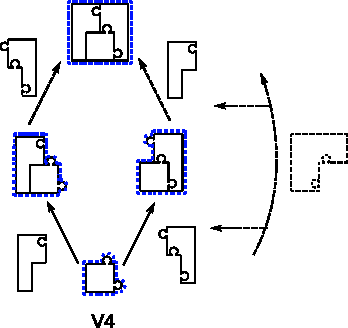
\includegraphics[width=.4\textwidth]{v4.pdf}
 \caption{V4 introduces multiple inheritance. For brevity we omit the factories/builders for the upper arrows.}
 \label{fig:puzzle_v4}
\end{wrapfigure}
\
\begin{coqcode}
#\hbmixin{}# SemiRing_of_Monoid A Monoid.axioms.
  Record axioms := {
    one : A;
    mul : A -> A -> A;
    (* 7 axioms are omitted. *)
  }.
#\hbend{}#.

#\hbfactory{}# Ring_of_AbelianGroup A
    AbelianGroup.axioms.
  Record axioms := {
    (* 2 operators and 5 axioms are omitted. *)
  }.
  ..
#\hbend{}#.
\end{coqcode}

Since semirings and Abelian groups do not inherit from each other,
the definition of semirings and Abelian groups are quite similar:
\begin{coqcode}
Module SemiRing.
Record axioms (T : Type) : Type := Class {
  Monoid_of_Type_mixin : Monoid_of_Type.axioms T;
  SemiRing_of_Monoid_mixin : SemiRing_of_Monoid.axioms T Monoid_of_Type_mixin; }.
Structure type : Type := Pack { sort : Type; class : axioms sort; }.
End SemiRing.
\end{coqcode}
We define implicit coercions from the semiring structure to the carrier
and the monoid structure, and we lift semiring operators and axioms as follows:
\begin{coqcode}
Coercion SemiRing.sort : SemiRing.type >-> Sortclass.
Coercion SemiRing_to_Monoid : SemiRing.type >-> Monoid.type.

Definition one {T : SemiRing.type} : T := ... .
Definition mul {T : SemiRing.type} : T -> T -> T := ... .
(* 7 semiring axioms are omitted. *)
\end{coqcode}

The class record is defined by gathering the monoid, Abelian group, and
semiring \mixins{}. Since the rings inherit from monoids, semirings, and
Abelian groups, we define implicit coercions from the ring structure to those
three structures.
\begin{coqcode}
Module Ring.
Record axioms (T : Type) : Type := Class {
  Monoid_of_Type_mixin : Monoid_of_Type.axioms T;
  SemiRing_of_Monoid_mixin : SemiRing_of_Monoid.axioms T Monoid_of_Type_mixin;
  AbelianGroup_of_Monoid_mixin : AbelianGroup_of_Monoid.axioms T Monoid_of_Type_mixin; }.
Structure type : Type := Pack { sort : Type; class : axioms sort; }.
End Ring.

Coercion Ring.sort : Ring.type >-> Sortclass.
Coercion Ring_to_Monoid : Ring.type >-> Monoid.type.
Coercion Ring_to_SemiRing : Ring.type >-> SemiRing.type.
Coercion Ring_to_AbelianGroup : Ring.type >-> AbelianGroup.type.
\end{coqcode}

\subsection{Linking structures and instances via Canonical Structures}

The mechanism of Canonical Structures~\cite{DBLP:conf/itp/MahboubiT13,Saibi99phd}
lets the user extend the elaborator of Coq. This software component
takes in input a term as written by the user and has to infer all the missing
piece of information that is necessary in order to make the term well typed.

A first example of elaboration that requires canonical structures is \(0 + 1\).
After removing all syntactic facilities, the underlying Coq term is
\coq{(add _ (zero _)) (one _)} where \coq{_} stands for an implicit piece
of information to be inferred and the constants \coq{add} and \coq{zero} come
from the monoid structure while \coq{one} comes from semirings.
When the term is type checked each \coq{_} is replaced by a unification
variable written $?_v$.
Respectively, the head and the argument of the top application
can be typed as follows:
\begin{coqcode}
  add #$?_{\texttt{M}}$# (zero #$?_{\texttt{M}}$#) : Monoid.sort #$?_{\texttt{M}}$# -> Monoid.sort #$?_{\texttt{M}}$#
  one #$?_{\texttt{SR}}$# : SemiRing.sort #$?_{\texttt{SR}}$#
\end{coqcode}
where \(?_{\texttt{M}}~\coq{: Monoid.type}\) and
\(?_{\texttt{SR}}~\coq{: SemiRing.type}\).
In order to type check the application Coq has to unify \(\coq{Monoid.sort}~?_{\texttt{M}}\) with
\(\coq{SemiRing.sort}~?_{\texttt{SR}}\), which is not trivial: it amounts at
finding a structure that is both a monoid and a semiring, possibly the
smallest one~\cite[Sect.~4]{KSdraft}.
This piece of information can be inferred from the hierarchy and its inheritance
relation (Definition~\ref{def:subclass}) and we can tell Coq to exploit it by
declaring \coq{SemiRing_to_Monoid : SemiRing.type -> Monoid.type} as
canonical. With that hint Coq will pick \(?_{\texttt{M}}\) to be
\(\coq{SemiRing_to_Monoid}~?_{\texttt{SR}}\) as the canonical solution for this
unification problem.
In general, all the coercions between structures must be declared
as canonical. % to make this inference work.

Another relevant example of elaboration problem is \(- 1\), which hides the term \coq{(opp _) (one _)}.
Here \coq{opp} and \coq{one} are respectively from Abelian groups and semirings,
which do not inherit each other but whose smallest common substructure is
rings; thus we have to extend the unifier to solve a unification problem
\(\coq{AbelianGroup.sort}~?_{\texttt{AbG}}~\coq{= SemiRing.sort}~?_{\texttt{SR}}\) by instantiating \(?_{\texttt{AbG}}\) and \(?_{\texttt{SR}}\) with \(\coq{Ring_to_AbelianGroup}~?_{\texttt{R}}\) and \(\coq{Ring_to_SemiRing}~?_{\texttt{R}}\) respectively where \(?_{\texttt{R}}\) is a fresh unification variable of type \coq{Ring.type}.
This hint can be given as follows:% can be done by the following canonical declaration.
\begin{coqcode}
Canonical AbelianGroup_to_SemiRing (T : Ring.type) :=
  SemiRing.Pack (AbelianGroup.sort (Ring_to_AbelianGroup T)) (Ring.class T)).
\end{coqcode}

Similarly, one can apply an algebraic theory to an instance (an example) of that structure, e.g., \(2 \times 3\) where \(2\) and \(3\) have type \(\mathbb{Z}\).
The same mechanism of canonical structures let us extend the unifier to solve \(\coq{SemiRing.type}~? = \mathbb{Z}\).


%%%%%%%%%%%%%%%%%%%%%%%%%%%%%%%%%%%%%%%%%%%%%%%%%%%%%%%%%%%%%%%%%%%%%%%%%%%%
\section{The implementation in Coq-Elpi}\label{sec:implementation}

The implementation is based on the Elpi
extension language for Coq. In this section we introduce the features of the
programming language that came in handy in the development of \HB{} and
comment a few code snippets.

Coq-Elpi~\cite{CoqElpi} is a Coq plugin embedding
Elpi and providing an
extensive, high level, API to access and script the Coq system at the
vernacular level.
This API lives in the \elpi{coq} namespace and lets one easily declare
records, coercions, canonical structures, modules, implicit arguments, etc.
The most basic Coq data type exposed to Elpi is the one of references to global
declarations:

\begin{elpicode}
kind gref  type.                 % The data type of references to global terms
type indt  inductive -> gref.    % eg: Coq.Init.Datatypes.nat
type indc  constructor -> gref.  % eg: Coq.Init.Datatypes.O
type const constant -> gref.     % eg: Coq.Init.Peano.plus
\end{elpicode}

The arguments of the three constructors are opaque to Elpi, that can only use
values of these types via dedicated APIs. For example the API for declaring
an inductive type will generate a value of type \elpi{inductive} that
is printed as, for example, \elpi{«nat»}.

Elpi~\cite{DBLP:conf/lpar/DunchevGCT15} is a dialect
of $\lambda$Prolog~\cite{Miller:2012:PHL:2331097}, an higher order
logic programming language that makes it easy to manipulate abstract syntax
tree with binders. Coq-Elpi takes full advantage of this capability by
representing Coq terms in Higher Order Abstract
Syntax~\cite{10.1145/53990.54010} style, reusing the binder of the programming
language in order to represent Coq's ones. Here is an excerpt of the data
type of Coq terms:

\begin{elpicode}
kind term type.                              % The data type of Coq terms
type global gref -> term.                    % eg: nat, O, S, plus, ...
type fun    term -> (term -> term) -> term.  % eg: fun x : t => b(x)
type app    list term -> term.               % eg: app [hd|args]
... % all other term constructors are omitted for brevity
\end{elpicode}

Note that the \elpi{fun} constructor holds a $\lambda$Prolog function.
In this syntax the Coq term \coq{(fun x : nat => x x)} becomes
\elpi{(fun (global (indt «nat»)) x\ app[x, x])} where \elpi{x\} binds \elpi{x}
in the body of the function. Substitution of a bound variable for a term
can be computed by applying a term (of function type) to an argument.

Data types with binders are also used as input to high level APIs that build
terms behind the scenes. For example a Coq record is just an inductive type
and the API to declare one must allow the type of a field to depend on the
fields that comes before it. Note that the \elpi{field} constructor
takes a coercion flag, the name of the field, its type and binds a term
in the remaining record declaration.

\begin{elpicode}
kind indt-decl type.              % The type of an inductive type declaration
type record      string -> term -> string -> record-decl -> indt-decl.
type field       bool -> string -> term -> (term -> record-decl) -> record-decl.
type end-record  record-decl.
... % constructors for non-record inductive types are omitted for brevity

external pred coq.env.add-indt i:indt-decl, o:inductive.
external pred coq.CS.canonical-projections i:inductive, o:list (option constant).
\end{elpicode}

The \elpi{pred} keyword documents types and modes (input or output) of the
arguments of a predicate, while \elpi{external} signals that the
predicate is a builtin (in other words it is implemented in
OCaml rather than $\lambda$Prolog).

We comment these two builtin predicates and the \elpi{indt-decl} type
while looking at the code of \elpi{declare-structure} that is in charge
of scripting the following Coq code:% (given as a parameter \coq{axioms}):

\begin{coqcode}
Structure type : Type := Pack { sort : Type; class : axioms sort }.
\end{coqcode}

The following Elpi code builds the declaration, type checks it, adds it to the
Coq environment and finally returns the projections for the sort and the class
fields.% (it is handy to have them in the rest of the code).

\begin{elpicode}
pred declare-structure i:gref, o:term, o:term, o:term.

declare-structure ClassName Structure SortProjection ClassProjection :- std.do! [
  StructureDeclaration =
    record "type" {{ Type }} "Pack" (
      field tt "sort" {{ Type }} s\                        %\label{binder:sort}%
      field ff "class" (app [global ClassName, s]) _\
    end-record),
  coq.typecheck-indt-decl StructureDeclaration,
  coq.env.add-indt StructureDeclaration StructureName,     %\label{record:decl}%
  coq.CS.canonical-projections StructureName [some SortP, some ClassP],
  Structure = global (indt StructureName),
  SortProjection = global (const SortP),
  ClassProjection = global (const ClassP),
].
\end{elpicode}

Note that the binder \elpi{s\} at line \ref{binder:sort} lets one mention
the first field in the type of the second.
The syntax \elpi{{{ Type }}} is a quotation: it lets
one use the syntax of Coq to write an Elpi expression of type \elpi{term}.
The API \elpi{coq.CS.canonical-projections} lets us find the projections
automatically generated by Coq for a given record.
The last detail worth mentioning is that this program makes no use of
backtraking: the \elpi{std.do!} combinator signals that.

In the simple case of the structure record, the number of fields, and hence
the number of binders, is fixed. On the contrary the class record has one
field per \mixin{} and each of them can depend on the previous ones.
In order to synthesize terms with binders in an inductive fashion (using
a recursive predicate) $\lambda$Prolog lets one postulate fresh nominal
constants using the \elpi{pi} operator and attach to the
nominal some knowledge in the form of a clause via the \elpi{=>} operator.
This process is called binder mobility: the binder is moved from
the data (that we are building) to the program (the context of the
current computation).
This feature is key to the following code that synthesizes the
declaration of the fields of the class record.

\begin{elpicode}
pred synthesize-fields.field-for-mixin i:mixinname, o:term.
pred synthesize-fields i:list mixinname, i:term, o:record-decl.

synthesize-fields [] _ Decl :- Decl = end-record.
synthesize-fields [M|ML] T Decl :- std.do! [
  get-mixin-modname M ModName, Name is ModName ^ "_mixin",                          %\label{craft:name}%
  dep1 M Deps,                                         %\label{deps:fetch}%
  std.map Deps synthesize-fields.field-for-mixin Args, %\label{deps:satisfy}%
  Type = app[ global M, T | Args ],                    %\label{build:type}%
  Decl = (field ff Name Type f\ Fields f),
  pi m\                                                %\label{postulate:m}%
    synthesize-fields.field-for-mixin M m =>           %\label{postulate:satisfy}%
    synthesize-fields ML T (Fields m)                  %\label{rec:call}%
].
\end{elpicode}

The first predicate \elpi{synthesize-fields.field-for-mixin} is used
to link a \mixin{} to a nominal that corresponds to the record field
for that mixin. It has no clauses in the base program but some clauses
are added dynamically by \elpi{synthesize-fields}.

The second predicate proceeds by recursion on the (topologically sorted) list of \mixins{},
and terminates when the list is empty. If the list contains a \mixin{} \elpi{M}
then it crafts a \elpi{Name} for it (line~\ref{craft:name}),
fetches its dependencies (line~\ref{deps:fetch}) and
finds the (previously declared) record fields holding these \mixins{}
(line~\ref{deps:satisfy}).
The \elpi{(std.map L1 P L2)} predicate relates the two lists \elpi{L1} and
\elpi{L2} point wise using the predicate \elpi{P}.

Line~\ref{build:type} builds the type of the field: the \mixin{} name applied
to the type (sort) and all its dependencies.
Note that the \elpi{Fields} variable, representing the declaration of the
next fields, is under the binder for \elpi{f} (the current field).
In order to make the recursive call under that binder (line~\ref{rec:call})
and recursively process \elpi{ML} we postulate a nominal
\elpi{m} (line~\ref{postulate:m}) that is a term satisfying any
future dependency on the current \mixin{} (line~\ref{postulate:satisfy})
and we replace \elpi{f} by \elpi{m} in \elpi{Fields} by writing
\elpi{(Fields m)}.


% The code of \elpi{synthesize-fields} makes an idiomatic use
% of \elpi{=>} in $\lambda$Prolog: the current program is temporarily
% extended with a clause.
%
% \marginpar{this may go}The same operation, but with a persistent
% effect, is made available by Coq-Elpi via a dedicated API to extend
% data bases. A data base is a named set of clauses and
% commands are typically built by accumulating specific clauses on top
% of a data base. Here an excerpt of the \verb+hierarchy.db+ data base and
% of the \elpi{declare_mixin} command. Text between \verb+lp:{{+ and \verb+}}+
% is Elpi code embedded in a Coq file. All the vernacular commands beginning
% with \coq{Elpi} are provided by the Coq-Elpi plugin.
%
% \begin{coqcode}
% Elpi Db hierarchy.db lp:{{
%   pred dep1 o:mixinname, o:list mixinname.
%   ... % for brevity we omit class and join
% }}.
% Elpi Command declare_mixin.
% Elpi Accumulate Db hierarchy.db.
% Elpi Accumulate lp:{{
%   main [str S] :- !, std.do! [
%     coq.locate S M,
%     coq.env.typeof M Ty,
%     gather-mixin-dendencies Ty [] ML, % implementation omitted for brevity
%     coq.elpi.accumulate "hierarchy.db" (clause _ _ (dep1 M ML)),
%     ...
%   ].
%   main _ :- coq.error "Usage: declare_mixin <mixin>".
% }}.
% \end{coqcode}
%
% Line 11 computes the dependencies of \mixin{} \elpi{M} given
% its type and line 12 crafs a clause for \elpi{dep1} and
% adds it to the data base \elpi{"hierarchy.db"}.
%
%%%%%%%%%%%%%%%%%%%%%%%%%%%%%%%%%%%%%%%%%%%%%%%%%%%%%%%%%%%%%%%%%%%%%%%%%%%%%
%\section{Benchmark}
%if we can port ssralg, or not... It would be nice, but maybe its a bit late.

%%%%%%%%%%%%%%%%%%%%%%%%%%%%%%%%%%%%%%%%%%%%%%%%%%%%%%%%%%%%%%%%%%%%%%%%%%%%%
\section{Related work}
The most closely related work is the one about Packed Classes~\cite{DBLP:conf/tphol/GarillotGMR09} on which we
build. The main differences are that \HB{} is a higher level language
that is compiled down to (flat) Packed Classes. The systematic use of
\factories{} makes the user interface of a hierarchy stable under the insertion of
structures, a property that Packed Classes lacks.
Finally many of the intricacies of Packed Classes are hidden to the user by
the compilation step, in particular creating all the necessary coercions and canonical structure declarations,
especially in the case of diamonds or when merging several libraries, which used to cause the need for \textit{a posteriori}
validation of a hierarchy design~\cite{KSdraft}. It also opens the way
to automatically detect and solve problems tied to non judgmental commutative diagrams when forgetting
structure~\cite{affeldt:hal-02463336}.


In~\cite{CaretteCombinators} Carette and O'Connor describe the language of
Theory Presentation Combinators that can be used to describe a hierarchy of
algebraic structures.
They focus on the categorical semantics of the language that is built upon
the category of context.
They do not describe any actual compilation to the language of a mainstream
interactive prover, indeed they claim their language to be mostly type theory
independent. We know they considered targeting type theory and the language
of unification hints~\cite{10.1007/978-3-642-03359-9_8}
(a super set of the one of Canonical Structures),
but we could not find any written trace of that. Language wise they provides
keywords such as \verb+combine+ and \verb+over+ to share (reuse) a property
when defining a new structure. For example in order to avoid restating
the commutativity property when defining Abelian groups they combine
a commutative monoid and a group forcing the subjacent monoid to coincide: %
\verb-CommutativeGroup := combine CommutativeMonoid , Group over Monoid.-
In our language \HB{} the same role is played by \emph{\mixins{}}.
A \mixin{} lets one write once and for all a property and abstract it over types
and operations so that it can be reused in all the structures that need it.
One operation \HB{} allows for but that does not seem to be possible in the
setting of Presentation Combinators is the one of replacing an axioms with a
lemma and vice versa. As shown in \autoref{subsec:evolution} \HB{} supports
that.

The MMT system~\cite{RABE20131} provides a framework to describe formal
languages in a logical framework, providing good support for binders and
notations. It also provides an expressive module system to organize
theories and express relations among them in the form of functors.
At the time of writing
it provides limited support for elaborating user input taking systematic
advantage of the contents of the theories. The elaborator can be extended
by the user writing Scala code, and in principle use the contents of the
libraries to make sense of an incomplete expressions, but no higher level
language or mechanism is provided.

The library of the Mizar system features a hierarchy of algebraic
structures~\cite{7733265}. In spite of lacking dependent types, Mizar
provides the concept of attributed types and adjectives
that can be used to describe the signature of structures as one would
do with a dependently typed record and their properties as
one would define a conjunctive predicate.
The Mizar language also provides the notion of cluster that is used
to link structures: by showing that property $P$ implies property $Q$
one can inform automation that structures characterized by $P$ are
instances of structures characterized by $Q$. The foundational theory of Mizar
features an extensional notion of equality that makes it easy
to share the signature or the properties of structures by just requiring
a proof of their equivalence that is in turn used by automation to treat
equivalent structures as equal.

The concepts of \factory{} and \builder{} presented here is akin to the
\verb-AbstractFactory- and \verb-Builder- pattern from "the Gang Of Four" design
patterns~\cite{gamma1995design} in the sense that \factories{} are used
to build an arbitrary number of objects (here \mixin{} instances).

%%%%%%%%%%%%%%%%%%%%%%%%%%%%%%%%%%%%%%%%%%%%%%%%%%%%%%%%%%%%%%%%%%%%%%%%%%%%
\section{Conclusion}
In this paper we design and implement \HB{}, a high level language to describe
hierarchies of algebraic structures. The implementation of \HB{} is
based on the Elpi extension language for the Coq system and is available
at \url{https://github.com/math-comp/hierarchy-builder}.
The implementation amounts to approximately a thousand lines of (commented)
Elpi code and tree hundred lines of Coq vernacular. It took less than one month
to implement \HB{} while it took several years of attempts and fruitful
discussions with the other developers of the Mathematical Components library
to design it, as well as Coq users and developers and members of Dagstuhl seminar 18341.
In particular, discussions with Georges Gonthier, Assia Mahboubi and
Florent Hivert were instrumental in coining the concepts formalized here.

The \HB{} language is only loosely tied to Coq or even Type Theory.
We believe it could be adopted with no major change to other tools. Indeed the
properties and invariants that link \factories{}, \mixins{} and \classes{}
are key to rule out meaningless or ambiguous sentences and are not
specific to our logic setting. Moreover
most logics feature packing construction similar to records.
The compilation scheme we present in \autoref{sec:target-lang} is tied to dependent records,
that are available in Coq but also
in other provers based on Type Theory such a Matita~\cite{DBLP:conf/cade/AspertiRCT11}
and Lean~\cite{DBLP:conf/cade/MouraKADR15}.
Then, we could also have chosen telescopes~\cite{telescopes} or unbundled
classes~\cite{mathclasses}, instead of Canonical Structures as the target language for \HB{},
and we believe it would take only a minor effort to patch \coq{hierarchy-builder}.
Historically, Mathematical Components library, given the size and
the depth of the hierarchy, adopts Packed Classes because they offer a good
compromise between flexibility and performance~\cite[Section 8]{DBLP:conf/itp/MahboubiT13} in Coq.
One could instead use a system which provide comparable
performances for unbundled classes or other ways to implement \HB{}
(e.g. Unification Hints~\cite{10.1007/978-3-642-03359-9_8}).
It is a virtue of our work to provide a user language that is separate
from the implementation one, so we could in principle target any other
equally expressive language without the user noticing.


We leave to future work extending \HB{} to support structures parametrized
by structures such as the one of module over a ring.
We also leave to future
work the automatic synthesis of the notion of morphism between structures
of the hierarchy.

\bibliography{biblio}
\newpage
\appendix

\section{Coq reference}

\begin{coqcode}
Section OperationProperties.
Variable T : Type.
Variable e : T.
Variable inv : T -> T.
Variable op : T -> T -> T.
Variable add : T -> T -> T.

Definition left_id  := forall x, op e x = x.
Definition right_id := forall x, op x e = x.

Definition left_inverse := forall x, op (inv x) x = e.

Definition commutative := forall x y, op x y = op y x.
Definition associative := forall x y z, op x (op y z) = op (op x y) z.

Definition left_distributive  := forall x y z, op (add x y) z = add (op x z) (op y z).
Definition right_distributive := forall x y z, op x (add y z) = add (op x y) (op x z).
\end{coqcode}

\section{Proof of addrC}
\begin{coqcode}
Lemma addrC {R : Ring.type} : commutative (@add R).
Proof.
have innerC (a b : R) : (a + b) + (a + b) = (a + a) + (b + b).
  by rewrite -[a+b]mul1r -mulrDl mulrDr !mulrDl !mul1r.
have addKl (a b c : R) : a + b = a + c -> b = c.
  apply: can_inj (add a) (add (-a)) _ _ _.
  by move=> x; rewrite addrA addNr add0r.
have addKr (a b c : R) : b + a = c + a -> b = c.
  apply: can_inj (add ^~ a) (add ^~ (-a)) _ _ _.
  by move=> x; rewrite /= -addrA addrN addr0.
move=> x y; apply: addKl (x) _ _ _; apply: addKr (y) _ _ _.
by rewrite -!addrA [in RHS]addrA innerC !addrA.
Qed.
\end{coqcode}

\end{document}

%%% Local Variables:
%%% mode: latex
%%% TeX-master: "hb.tex"
%%% TeX-command-extra-options: "-shell-escape"
%%% ispell-local-dictionary: "english"
%%% End: